\section{Context Engine}
\label{sec:implementation:context-engine}

In \Cref{sec:design:bayesian-network,sec:design:context-engine}, the reason for introducing action nodes at the middle level of the Bayesian network and thus ``translating'' probabilities of gestures and rooms at the uppermost level to probababilities of actions is described. Modelling the Bayesian network in this way results in a modular design in which contextual information observed by different sensors can be independent. In the following we will briefly describe the realization of this design, which we refer to as the \emph{context engine}. We will also discuss the benefits of the engine.

\Cref{fig:implementation:context-engine} shows a class diagram of all clases and interfaces involved in the context engine. Below is a brief description of the classes and interface.

\begin{description}
\item[ContextualInformationProvider] Observes a delimited area of the context and provides information about the area to the \texttt{ContextRecognizer}. The provided information is encapsulated in a \texttt{ProvidedContextualInformation} model. Examples of \texttt{ContextualInformationProvider}s include the \texttt{GestureContextualInformationProvider} and the \texttt{PositionContextualInformationProvider} which provides information about the performed gesture and the room the user is in respectively. Providers encapsulate one or more nodes in the Bayesian network presented in \Cref{sec:design:bayesian-network}. It encapsulate a node at the middle level in the network and zero or more nodes at the uppermost level. For example, the \texttt{GestureContextualInformationProvider} encapsulates the Gesture and Gesture\_Action nodes. The providers are described in greater detail later in this section.
\item[ContextualInformationListener] Objects conforming to the interface can get a callback when a \texttt{ContextualInformationProvider} either has the necessary contextual information or fails to retrieve it. The \texttt{ContextRecognizer} pass these as anonymous classes in Java.
\item[ProvidedContextualInformation] Encapsulates information from a \texttt{ContextualInformationProvider}. The model contains the node which should be parent to the Action node, a node to apply evidence to and the soft evidence to apply to the node. The parent node, which resides at the middle level in the Bayesian network, and the node to apply evidence to can be the same.
\item[ContextRecognizer] The recognizer orchestrates the retrieval of contextual information from the providers. Because a provider is not required to provide its contextual information instantly, the recognizer will timeout and thus cancel the provider if it takes too long to deliver the information.
\item[ContextRecognizerListener] When recognition completes, the context recognizer informs a listener about the outcome. Objects conforming to the \texttt{ContextRecognizerListener} interface can be informed about the outcome.
\item[ContextOutcome] A context outcome encapsulates an action that can be triggered and the probability that the action should be triggered. Context outcomes are the result of performing context recognition. The outcomes are parsed to the object conforming to the \texttt{ContextRecognizerListener} interface.
\end{description}

Because the Baysian network is modelled to ``translate'' probabilities of states on the uppermost level to probabilities of actions in the system at the middle level, we can implement the contextual information providers to be entirely independent of each other have each provider encapsulate all the information it needs.
In order to use the provider, it is added to the context recognizer which needs to know nothing about the contextual information encapsulated but only the probabilities of the states, i.e. the \texttt{ProvidedContextualInformation}, as defined by the \texttt{ContextualInformationProvider} interface.

\begin{figure}[h!]
\centering
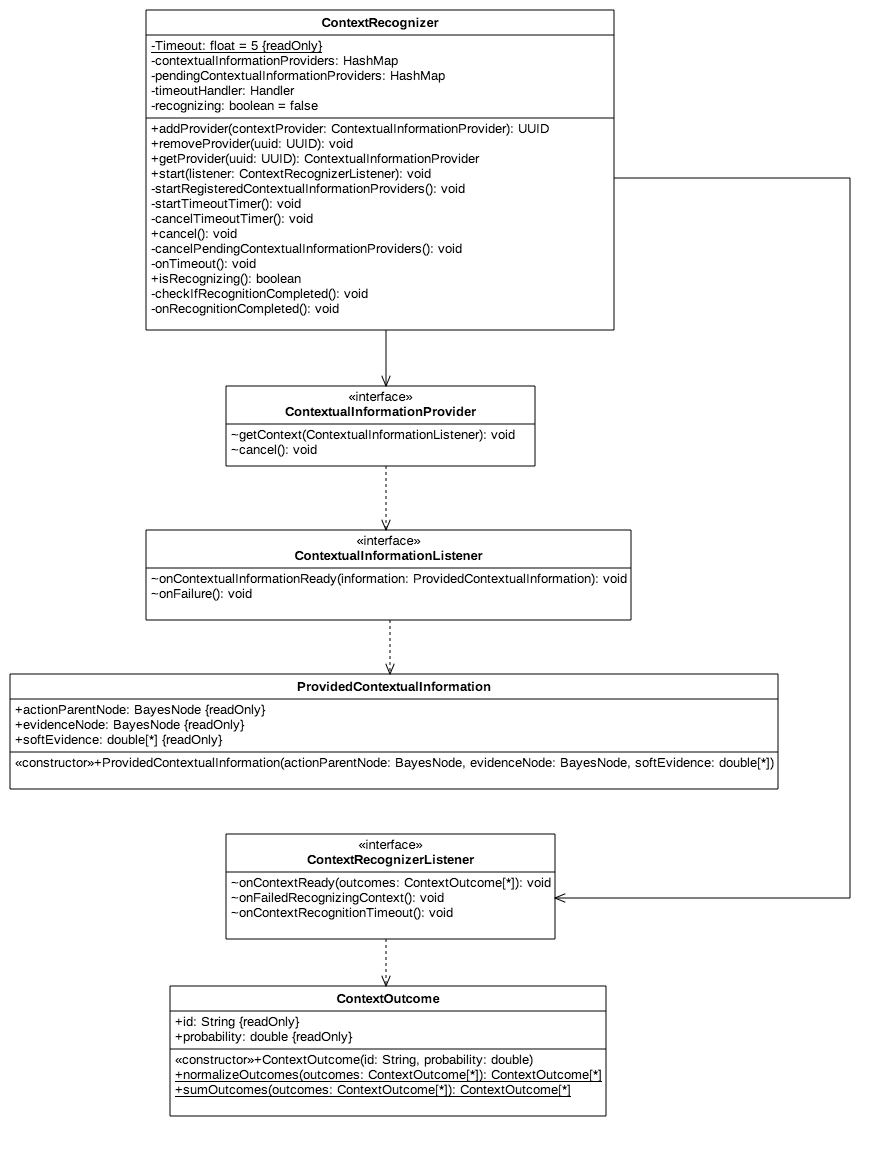
\includegraphics[width=\textwidth]{images/uml-context-engine}
\caption{Class diagram showing all classes and interfaces involved in the context engine.}
\label{fig:implementation:context-engine}
\end{figure}

\Cref{fig:implementation:context-engine:providers} shows a class diagram of the contextual information providers registered with the context recognizer in the prototype developed duing the project. Below is a brief description of the classes and interfaces.

\begin{description}
\item[Beacon] A representation of a beacon installed in a room. Beacons are retrieved from openHAB over HTTP using the REST API.
\item[Room] A representation of a room which the user can be in. Rooms are retrieved from openHAB over HTTP using the REST API.
\item[PositionManager] The manager continuously listens for changes to the users position using the Estimote SDK. Based on RSSI measurements received by the Estimote SDK, the manager determines which room the user is in.
\item[EventListener] Part of the \texttt{PositionManager}. Objects conforming to the interface can be informed when the manager registers the user in a room.
\item[GestureContextualInformationProvider] Encapsulates the Gesture and Gesture\_Action nodes in the Bayesian network presented in \Cref{sec:design:bayesian-network}. When gesture recognition ends, the provider is updated with the matches which it stores and use to compute the evidence when asked to provide its contextual information as described in \Cref{sec:design:bayesian-network:gesture-node-evidence}.
\item[PositionContextualInformationProvider] Encapsulates the Room and Room\_Action nodes in the Bayesian network. Based on the observations made by the \texttt{PositionManager}, the provider calculates probabilities for the user being in each room as described in \Cref{sec:design:bayesian-network:room-node-evidence}.
\end{description}

\begin{figure}[h!]
\centering
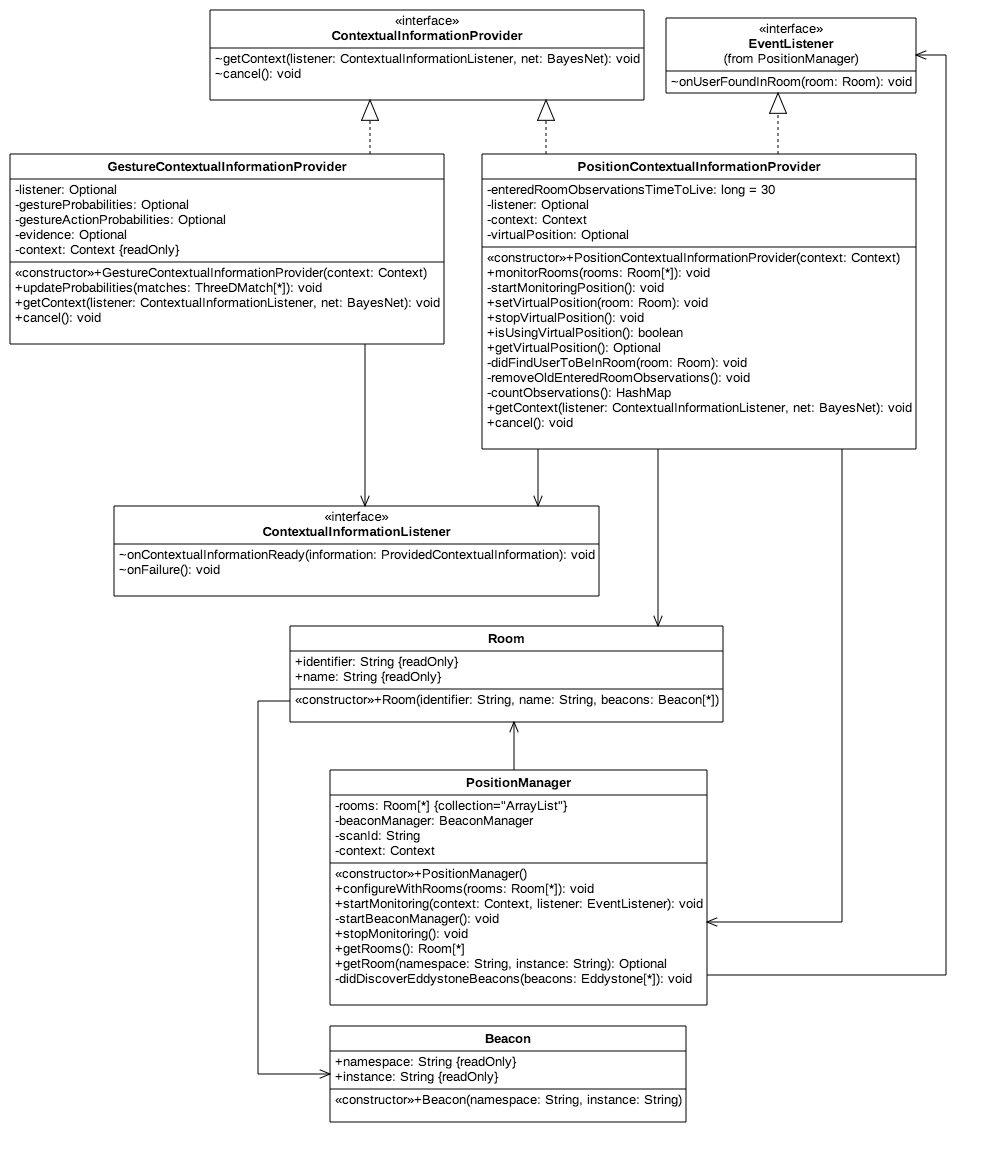
\includegraphics[width=\textwidth]{images/uml-context-engine-providers}
\caption{Class diagram showing the clases and interfaces involved in the providers.}
\label{fig:implementation:context-engine:providers}
\end{figure}

%%% Local Variables:
%%% mode: latex
%%% TeX-master: "../../master"
%%% End:
